\documentclass[a4paper,12pt]{report}

\usepackage{cmap}
\usepackage[T2A]{fontenc}
\usepackage[utf8]{inputenc}
\usepackage[english,russian]{babel}
\usepackage{listings}
\usepackage{amsmath}
\usepackage{float}
\usepackage{csquotes}

% \usepackage{titlesec}
% \newcommand{\sectionbreak}{\clearpage}

\usepackage{graphicx}
\graphicspath{ {./images/} }

\usepackage{xcolor}
% \usepackage{courier}

\definecolor{buzzlightyear}{HTML}{8757A5}
\definecolor{grass}{HTML}{738D06}
\definecolor{literal}{HTML}{F18A2B}
\definecolor{commentcolor}{HTML}{8E908B}

\lstdefinestyle{habrstyle}{
    backgroundcolor=\color{white},   
    commentstyle=\color{commentcolor},
    keywordstyle=\bfseries\color{buzzlightyear},
    numberstyle=\tiny\color{commentcolor},
    stringstyle=\color{grass},
    basicstyle=\ttfamily\footnotesize,
    breakatwhitespace=false,         
    breaklines=true,                 
    captionpos=b,                    
    keepspaces=true,                 
    numbers=left,                    
    numbersep=5pt,                  
    showspaces=false,                
    showstringspaces=false,
    showtabs=false,                  
    tabsize=4
}

\lstset{style=habrstyle}

\author{Луняк Николай}
\title{Лабораторная работа 1}
\date{\today}

\begin{document}
    \maketitle
    \tableofcontents
    \listoffigures
    \lstlistoflistings
    
    \chapter{Проверка}
    
    Тут надо просто проверить, что ноутбуки запускаются. Да, запускаются.
    
    \begin{figure}[H]
        \centering
        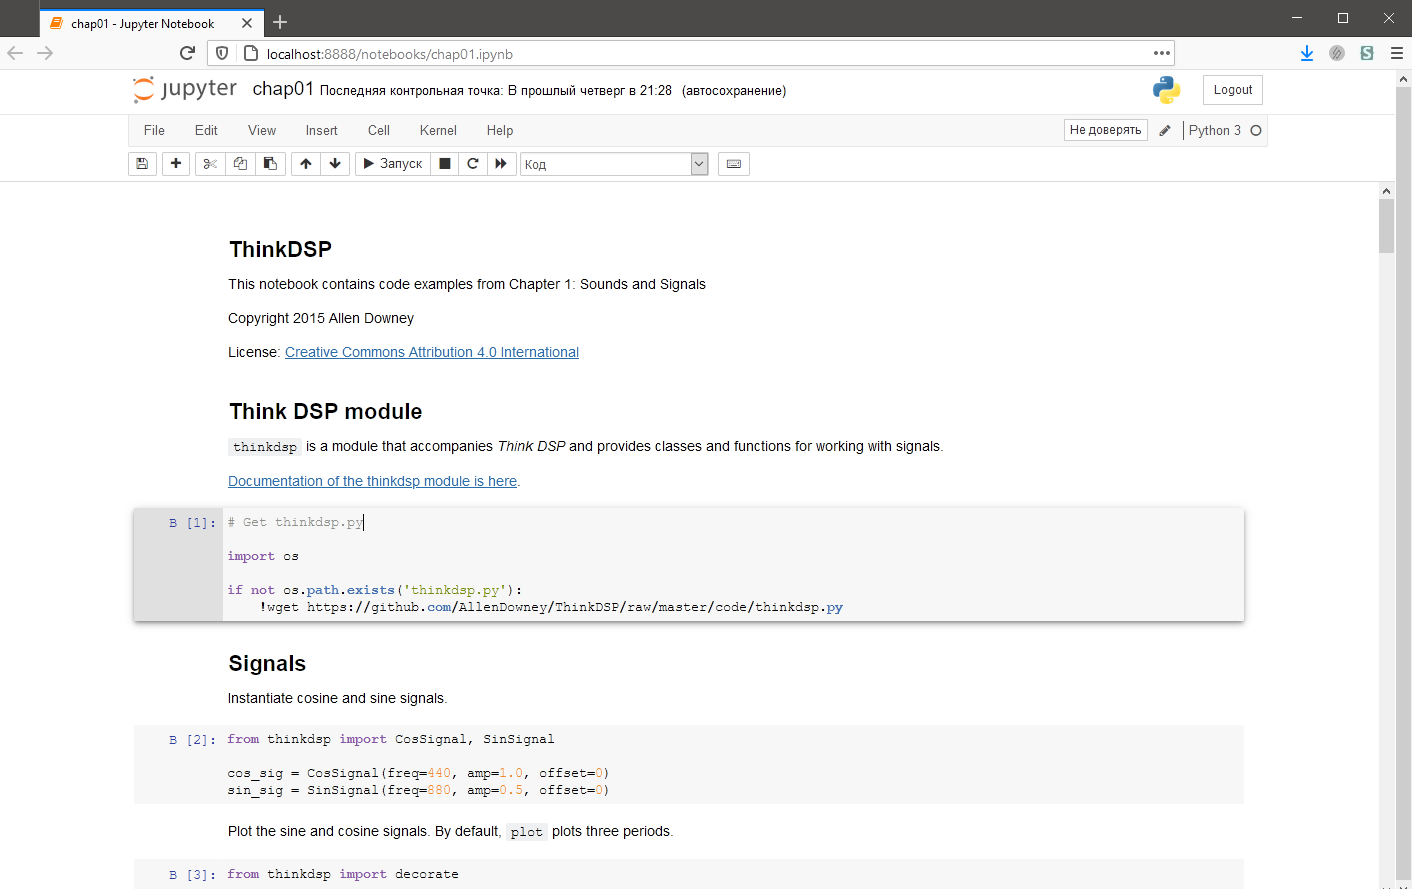
\includegraphics[width=\textwidth]{ex1_it_works.png}
        \caption{Работает}
        \label{fig:ex1_it_works}
    \end{figure}
    
    Но не все так гладко... Например, в коде ниже используется \texttt{aplay}, которого у меня нет, потому что я работаю на Windows.
    
\begin{lstlisting}[language=Python,caption=Использование \texttt{aplay}]
from thinkdsp import play_wave
play_wave(filename='temp.wav', player='aplay')
\end{lstlisting}
    
    Я попробовал использовать \texttt{ffplay}, который у меня есть, и звук, действительно, стал проигрываться... но он так никогда и не закончил это делать и notebook завис на одной команде. Пришлось перезапускать.
    
    \chapter{Простая обработка}
    \section{Получение звука}
    
\begin{lstlisting}[language=Python,caption=Загрузка звука]
from thinkdsp import read_wave
wave = read_wave(
    'Sounds/557274__johnnie-holiday__dark-ambience_cut.wav'
)
\end{lstlisting}

    По какой-то причине скаченный файл содержал 3 канала, из-за чего \texttt{play\_wave()} не могла его загрузить. Пришлось открыть Audacity и пересохранить файл руками (и там же я его и обрезал до половины секунды).
    
\begin{lstlisting}[language=Python,caption=Визуализация]
from thinkdsp import decorate
segment = wave.segment(0, wave.duration)
segment.plot()
decorate(xlabel='Time (s)')
\end{lstlisting}

    \begin{figure}[H]
        \centering
        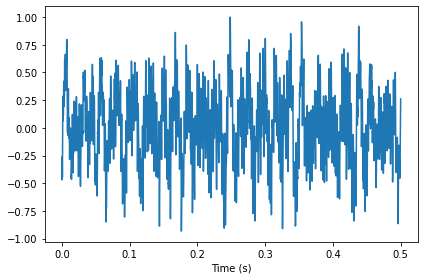
\includegraphics[width=0.75\textwidth]{ex2_source_waveform.png}
        \caption{Исходный звук}
        \label{fig:ex2_source_waveform}
    \end{figure}
    
    \section{Спектр}
    
\begin{lstlisting}[language=Python,caption=Спектр]
spectrum = segment.make_spectrum()
spectrum.plot()
decorate(xlabel='Frequency (Hz)')
\end{lstlisting}

    \begin{figure}[H]
        \centering
        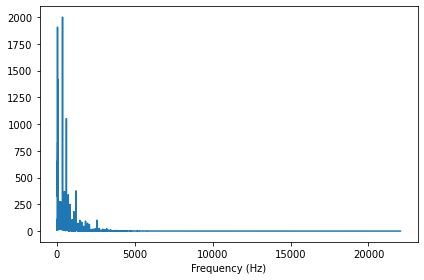
\includegraphics[width=0.75\textwidth]{ex2_spectrum.png}
        \caption{Спектр}
        \label{fig:ex2_spectrum}
    \end{figure}
    
\begin{lstlisting}[language=Python,caption=Улучшаем масштаб]
spectrum.plot(high=3000)
decorate(xlabel='Frequency (Hz)')
\end{lstlisting}

    \begin{figure}[H]
        \centering
        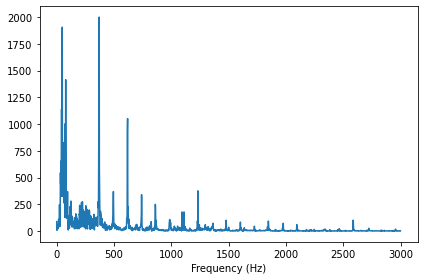
\includegraphics[width=0.75\textwidth]{ex2_spectrum_better.png}
        \caption{Улучшили масштаб}
        \label{fig:ex2_spectrum_better}
    \end{figure}
    
    Чем больше частот, тем более богатым считается тембр.

    В первый раз я взял звук под названием 445999\_\_breviceps\_\_fart-2, и его спектр оказался чуть ли не шумом. После небольшой фильтрации я вообще получил тишину. Получается, подобные звуки - сами по себе шум, а в соответствии с определением выше, они могут считаться очень богатыми.
    
    \section{Фильтрация}
    
\begin{lstlisting}[language=Python,caption=Делаем \texttt{low\_pass}]
spectrum.low_pass(1300)
spectrum.plot(high=1300)
decorate(xlabel='Frequency (Hz)')
\end{lstlisting}

    \begin{figure}[H]
        \centering
        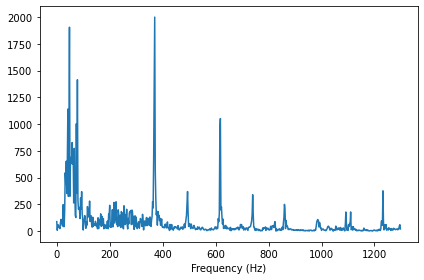
\includegraphics[width=0.75\textwidth]{ex2_low_pass.png}
        \caption{После \texttt{low\_pass}}
        \label{fig:ex2_low_pass}
    \end{figure}
    
\begin{lstlisting}[language=Python,caption=Финальный результат]
filtered = spectrum.make_wave()
filtered.normalize()
filtered.plot()
decorate(xlabel='Time (s)')
\end{lstlisting}

    \begin{figure}[H]
        \centering
        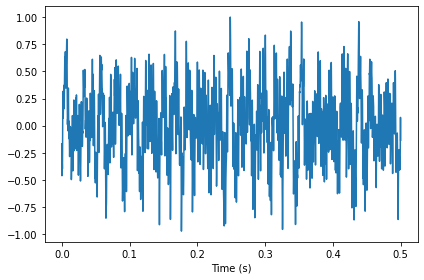
\includegraphics[width=0.75\textwidth]{ex2_final_filtered.png}
        \caption{Финальный результат}
        \label{fig:ex2_final_filtered}
    \end{figure}

    Звучит это все дело в сравнении с оригиналом так, как если бы на пути от источника звука до \textquote{нас} образовалась какая-то стена.
    
    \chapter{Комбинирование}
    \section{Кратные частоты}
    
\begin{lstlisting}[language=Python,caption=Создаем 2 сигнала]
from thinkdsp import CosSignal, SinSignal

cos_sig = CosSignal(freq=440,     amp=1.0, offset=0)
sin_sig = SinSignal(freq=440 * 3, amp=0.7, offset=0)

cos_sig.plot()
decorate(xlabel='Time (s)')

sin_sig.plot()
decorate(xlabel='Time (s)')
\end{lstlisting}

    \begin{figure}[H]
        \centering
        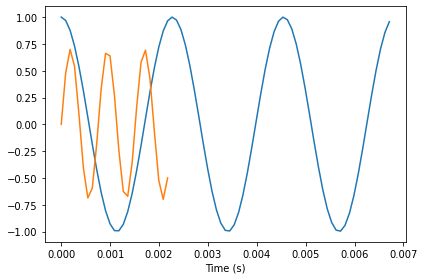
\includegraphics[width=0.75\textwidth]{ex3_creating_2_signals.png}
        \caption{Смотрим на 2 сигнала}
        \label{fig:ex3_creating_2_signals}
    \end{figure}
    
\begin{lstlisting}[language=Python,caption=Суммируем 2 сигнала]
mix = sin_sig + cos_sig
mix.plot()
decorate(xlabel='Time (s)')
\end{lstlisting}

    \begin{figure}[H]
        \centering
        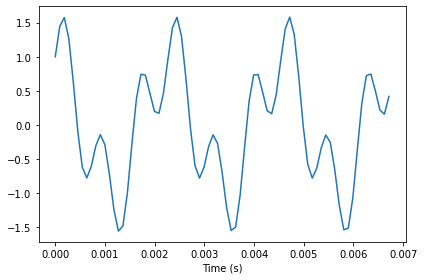
\includegraphics[width=0.75\textwidth]{ex3_sum_of_2_multiples.png}
        \caption{Смотрим на сумму 2 сигналов}
        \label{fig:ex3_sum_of_2_multiples}
    \end{figure}
    
\begin{lstlisting}[language=Python,caption=Смотрим на спектр 2 сигналов]
spectrum = wave.make_spectrum()
spectrum.plot(high=2000)
decorate(xlabel='Frequency (Hz)')
\end{lstlisting}

    \begin{figure}[H]
        \centering
        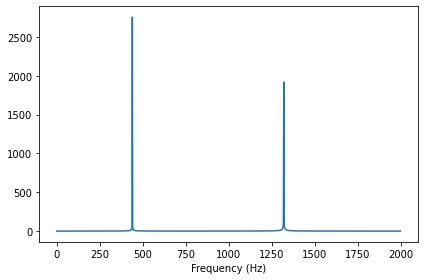
\includegraphics[width=0.75\textwidth]{ex3_spectrum_of_2_multiples.png}
        \caption{Смотрим на спектр суммы}
        \label{fig:ex3_spectrum_of_2_multiples}
    \end{figure}
    
    На слух это все звучит... ну нормально. Звук как звук. Относительно приятный.
    
    \section{Вносим что-то несочетающееся}
    
\begin{lstlisting}[language=Python,caption=Примешиваем некратную частоту]
one_more_cos_sig = CosSignal(
    freq=440 * 2.1315,
    amp=1.0,
    offset=0
)

one_more_mix = mix + one_more_cos_sig
one_more_mix.plot()
decorate(xlabel='Time (s)')
\end{lstlisting}

    \begin{figure}[H]
        \centering
        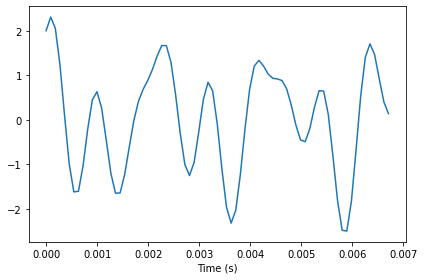
\includegraphics[width=0.75\textwidth]{ex3_adding_non_multiple.png}
        \caption{Вместе с некратной}
        \label{fig:ex3_adding_non_multiple}
    \end{figure}
    
\begin{lstlisting}[language=Python,caption=Смотрим спектр]
one_more_spectrum = one_more_wave.make_spectrum()
one_more_spectrum.plot(high=2000)
decorate(xlabel='Frequency (Hz)')
\end{lstlisting}

    \begin{figure}[H]
        \centering
        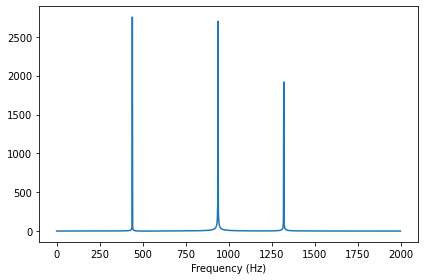
\includegraphics[width=0.75\textwidth]{ex3_spectrum_of_non_multiples.png}
        \caption{Спектр}
        \label{fig:ex3_spectrum_of_non_multiples}
    \end{figure}
    
    Этот звук уже больше походит на звук ошибки на каком-то космическом корабле.
    
    \section{Генерация}
    
    Хочется посмотреть, что будет, если взять много частот. Для этого я написал функцию \texttt{generate\_compound()}, которой надо передать количество частот и правило генерации $i$-ой частоты.
    
\begin{lstlisting}[language=Python,caption=Генерация]
def generate_compound(components_count, get_next_frequency):
    mix = CosSignal(
        freq=get_next_frequency(0),
        amp=1.0,
        offset=0
    )
    
    for it in range(2, components_count, 2):
        frequency = get_next_frequency(it)
        mix += CosSignal(
            freq=frequency,
            amp=1.0/(it + 1)**2,
            offset=0
        )
        
    for it in range(1, components_count, 2):
        frequency = get_next_frequency(it)
        mix += SinSignal(
            freq=frequency,
            amp=1.0/(it + 1)**2,
            offset=0
        )
    
    return mix.make_wave(
        duration=0.5,
        start=0,
        framerate=11025
    )
\end{lstlisting}

    Пользоваться этим можно так:
    
\begin{lstlisting}[language=Python,caption=Создаем \texttt{Wave}'ы]
import random

wave_multiples = generate_compound(
    10, 
    lambda it: 440 * (it + 1)
)

wave_non_multiples = generate_compound(
    10,
    lambda it: 440 * random.uniform(1, 5)
)
\end{lstlisting}

\begin{lstlisting}[language=Python,caption=Смотрим кратные]
wave_multiples.plot()
decorate(xlabel='Time (s)')
\end{lstlisting}

    \begin{figure}[H]
        \centering
        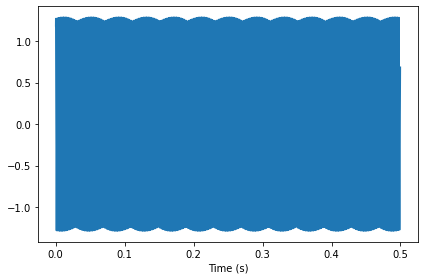
\includegraphics[width=0.75\textwidth]{ex3_visualizing_multiples.png}
        \caption{Смотрим кратные}
        \label{fig:ex3_visualizing_multiples}
    \end{figure}
    
\begin{lstlisting}[language=Python,caption=Смотрим некратные]
wave_non_multiples.plot()
decorate(xlabel='Time (s)')
\end{lstlisting}

    \begin{figure}[H]
        \centering
        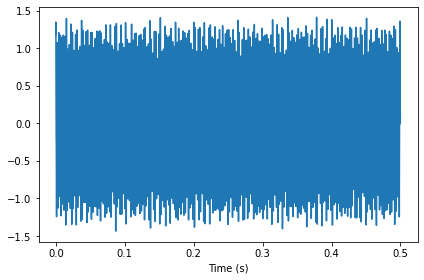
\includegraphics[width=0.75\textwidth]{ex3_visualizing_non_multiples.png}
        \caption{Смотрим некратные}
        \label{fig:ex3_visualizing_non_multiples}
    \end{figure}
    
    Ну и сами спектры.
    
\begin{lstlisting}[language=Python,caption=Смотрим спектр кратных]
spectrum_multiples = wave_multiples.make_spectrum()
spectrum_multiples.plot()
decorate(xlabel='Frequency (Hz)')
\end{lstlisting}

    \begin{figure}[H]
        \centering
        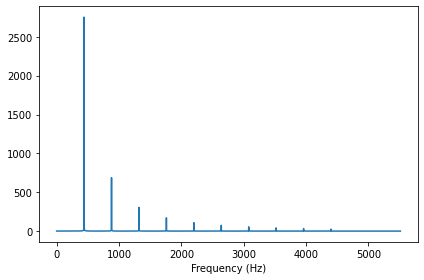
\includegraphics[width=0.75\textwidth]{ex3_spectrum_of_multiples_series.png}
        \caption{Смотрим спектр кратных}
        \label{fig:ex3_spectrum_of_multiples_series}
    \end{figure}
    
\begin{lstlisting}[language=Python,caption=Смотрим спектр некратных]
spectrum_non_multiples = wave_non_multiples.make_spectrum()
spectrum_non_multiples.plot()
decorate(xlabel='Frequency (Hz)')
\end{lstlisting}

    \begin{figure}[H]
        \centering
        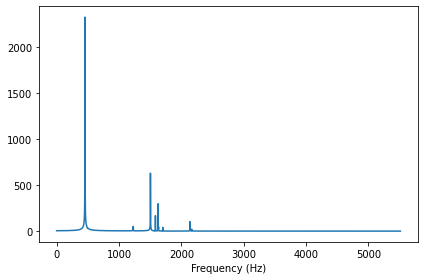
\includegraphics[width=0.75\textwidth]{ex3_spectrum_of_non_multiples_series.png}
        \caption{Смотрим спектр некратных}
        \label{fig:ex3_spectrum_of_non_multiples_series}
    \end{figure}
    
    Полученные звуки различаются, и природа этой разнецы та же, что и у полученых ранее звуков. Первый звук кажется более цельным (одна нота, но проигранная на неком инструменте со своим особым тембром), в то время как второй звук явно состоит из каких-то частей.
    
    \chapter{Растяжение}

    Ну, тут все понятно.

\begin{lstlisting}[language=Python,caption=Растягиваем \texttt{Wave}]
def stretch(wave, stretch_factor):
    wave.framerate *= stretch_factor
\end{lstlisting}

\end{document}
